\section{Branches}

\subsection{Branches in a Nutshell}

\begin{frame}
  \frametitle{Branches in a Nutshell (1)}
  \begin{itemize}
  \item When you make a commit, Git stores a commit object that contains a pointer to the snapshot of the content you staged.
  \item This object also contains the author’s name and email address, the message that you typed, and pointers to the commit or commits that directly came before this commit (its parent or parents)
  \end{itemize}
  \begin{center}
    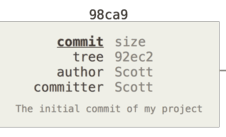
\includegraphics[width=0.7\linewidth]{figures/git-commit}
  \end{center}
commit-and-tree
\end{frame}

\defverbatim[colored]\gitcommit{
  \begin{shcode}
    $ git add README test.rb LICENSE
    $ git commit -m 'The initial commit of my project'
  \end{shcode}
}

\begin{frame}
  \frametitle{Branches in a Nutshell (2)}
  \begin{itemize}
  \item let’s assume that you have a directory containing three files, and you stage them all and commit.
  \item Staging the files computes a checksum for each one (the SHA-1 hash we mentioned before), stores that version of the file in the Git repository (Git refers to them as blobs), and adds that checksum to the staging area:
  \end{itemize}
\gitcommit
  \begin{itemize}
  \item When you create the commit by running git commit, Git checksums each subdirectory and stores those tree objects in the Git repository. 
  \item Git then creates a commit object that has the metadata and a pointer to the root project tree so it can re-create that snapshot when needed.
  \end{itemize}
\end{frame}

\begin{frame}
  \frametitle{Branches in a Nutshell (3)}
  Your Git repository now contains five objects:
  \begin{itemize}
  \item three blobs (representing the contents of one of the three files)
  \item one tree that lists the contents of the directory and specifies which file names are stored as which blobs
  \item one commit with the pointer to that root tree and all the commit metadata.
  \end{itemize}
  \vspace{-1em}
  \begin{center}
    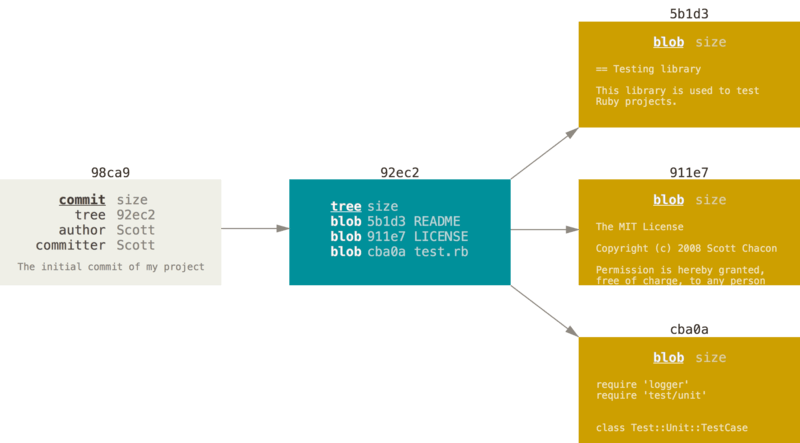
\includegraphics[width=0.9\linewidth]{figures/commit-and-tree}
  \end{center}
\end{frame}

\begin{frame}
  \frametitle{Branches in a Nutshell (4)}
If you make some changes and commit again, the next commit stores a pointer to the commit that came immediately before it.
  \vspace{1em}
  \begin{center}
    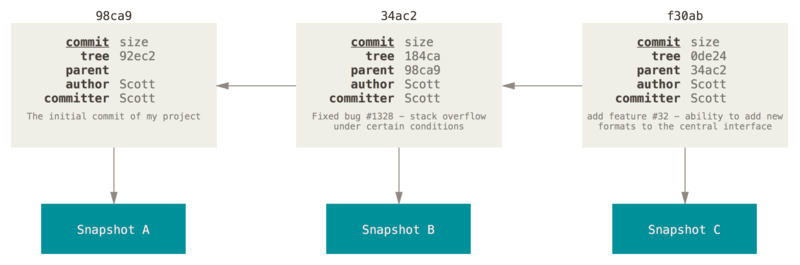
\includegraphics[width=\linewidth]{figures/commits-and-parents}
  \end{center}
\end{frame}

\subsection{Branches in action}

\begin{frame}
  \frametitle{Branches}

  A branch in Git is simply a lightweight movable pointer to one of these commits. By default, there is only one branch (called \texttt{master}) on a git repository.

  \begin{center}
    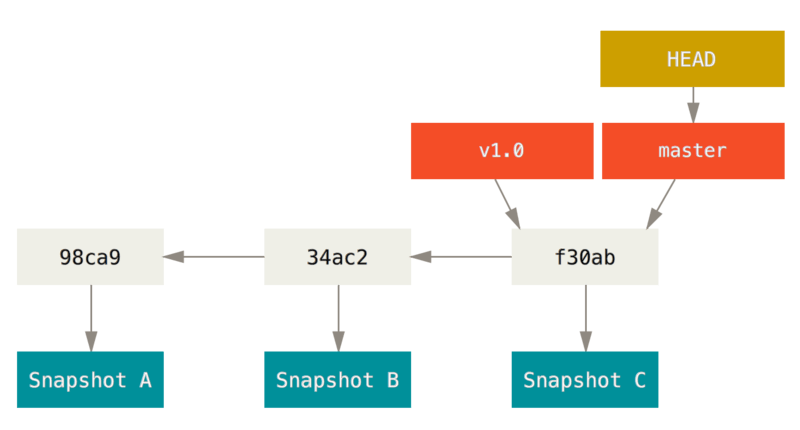
\includegraphics[width=\linewidth]{figures/branch-and-history}
  \end{center}

\end{frame}


\defverbatim[colored]\giteight{
  \begin{shcode}
      $ git branch testing
  \end{shcode}
}
\begin{frame}
  \frametitle{Branches (2)}

  You may create a new branch, to develop something new while keeping the
  master stable.

  \vspace{1em}

  \giteight

  \begin{center}
    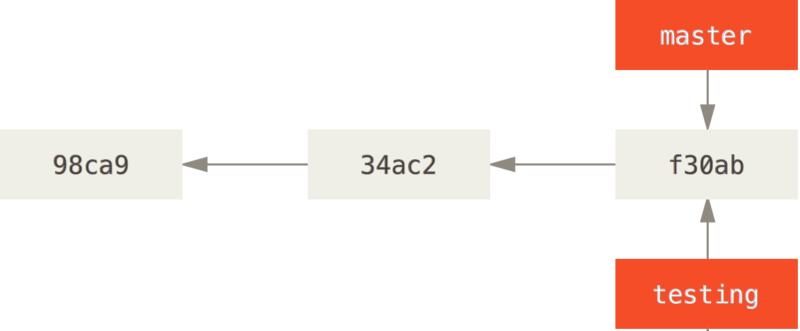
\includegraphics[width=0.9\linewidth]{figures/git-two-branches}
  \end{center}

\end{frame}

\begin{frame}
  \frametitle{Branches (3)}

  How does Git know what branch you’re currently on?\\
  It keeps a special pointer called \texttt{HEAD}

  \begin{center}
    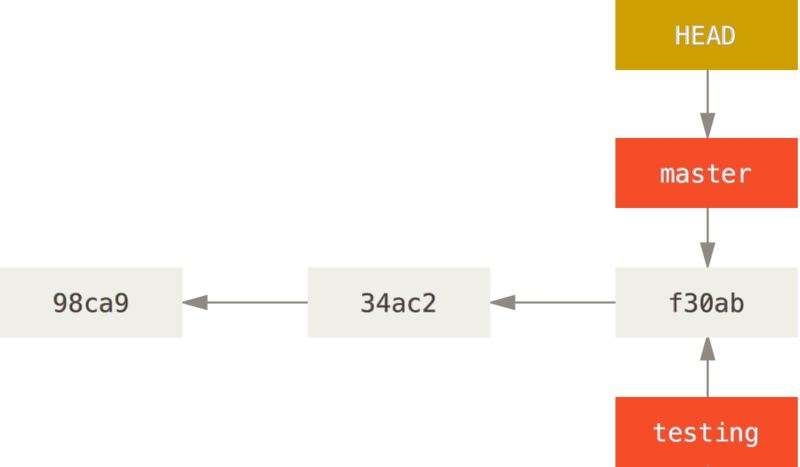
\includegraphics[width=0.7\linewidth]{figures/head-to-master}
  \end{center}
  
  \begin{alertblock}{Pay attention!}
    The git branch command only created a new branch - it didn't switch to that branch.
  \end{alertblock}
\end{frame}


\defverbatim[colored]\gitdecorate{
  \begin{shcode}
      $ git log --oneline --decorate
      f30ab (HEAD -> master, testing) add feature #32 - ability to add
      # new formats to the central interface
34ac2 Fixed bug #1328 - stack overflow under certain conditions
98ca9 The initial commit of my project
  \end{shcode}
}
\begin{frame}
  \frametitle{Branches (4)}

   You can easily see on which branch the \texttt{HEAD} is pointing by running a simple \texttt{git log} command that shows you where the branch pointers are pointing. This option is called \texttt{--decorate}.

  \gitdecorate
\end{frame}



\defverbatim[colored]\gitnine{
  \begin{shcode}
      $ git checkout testing
      Switched to a branch "testing"
  \end{shcode}
}

\subsection{Switching Branches}
\begin{frame}
  \frametitle{Switching Branches}

  To tell Git to consider a new branch as the default for commiting, use the
  \texttt{checkout} command:

  \gitnine

This moves \texttt{HEAD} to point to the \texttt{testing} branch.

\begin{center}
    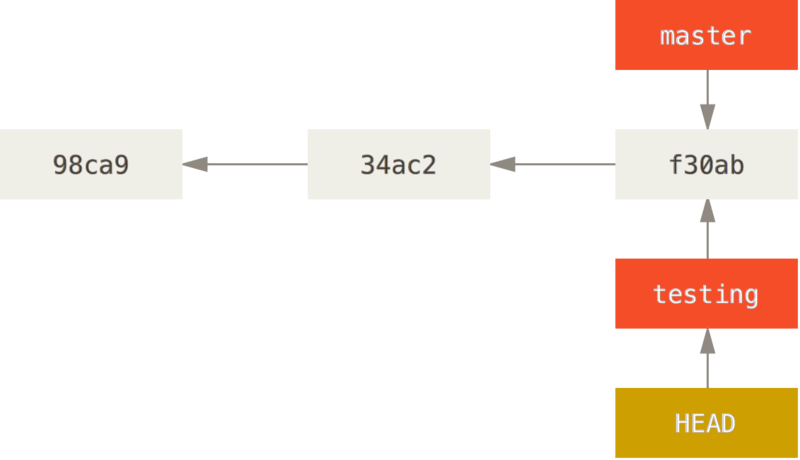
\includegraphics[width=0.7\linewidth]{figures/head-to-testing}
  \end{center}

\end{frame}


\defverbatim[colored]\gitcommitbranch{
  \begin{shcode}
      $ vim test.rb
      $ git commit -a -m 'made a change'
  \end{shcode}
}

\begin{frame}

  \frametitle{Switching Branches (2)}

  If you commit a change, only the marker \texttt{testing} will be modified:

  \gitcommitbranch

  \begin{center}
    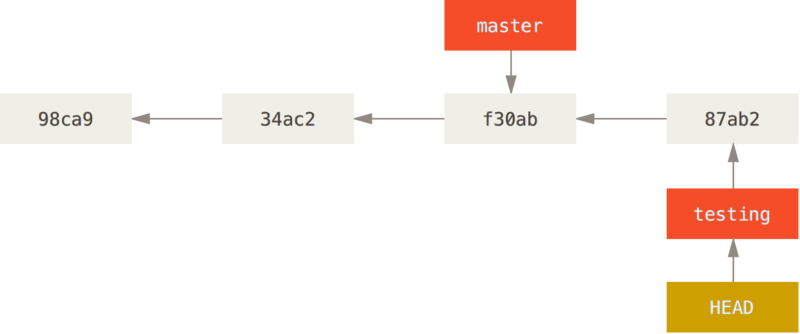
\includegraphics[width=0.8\linewidth]{figures/advance-testing}
  \end{center}

\end{frame}

\defverbatim[colored]\gitcheckoutmaster{
  \begin{shcode}
      $ git checkout master
  \end{shcode}
}
\begin{frame}
  \frametitle{Switching Branches (3)}

  If you commit a change, only the marker \texttt{testing} will be modified:

  \gitcheckoutmaster
  \vspace{-1em}
  \begin{center}
    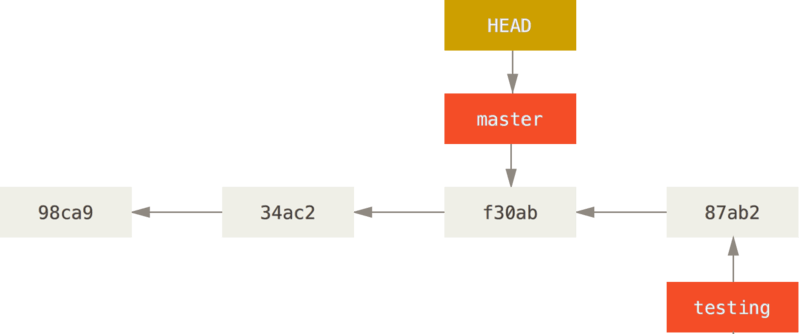
\includegraphics[width=0.7\linewidth]{figures/checkout-master}
  \end{center}
  \begin{alertblock}{Pay attention!}
  That command did two things. It moved the \texttt{HEAD} pointer back to point to the \texttt{master} branch, and it reverted the files in your working directory back to the snapshot that master points to. 
  \end{alertblock}
\end{frame}

\defverbatim[colored]\gitmorechanges{
  \begin{shcode}
      $ vim test.rb
      $ git commit -a -m 'made other changes'
  \end{shcode}
}
\begin{frame}
  \frametitle{Switching Branches (4)}
  Let’s make a few changes and commit again:
  \gitmorechanges
  \vspace{-1em}
  \begin{center}
    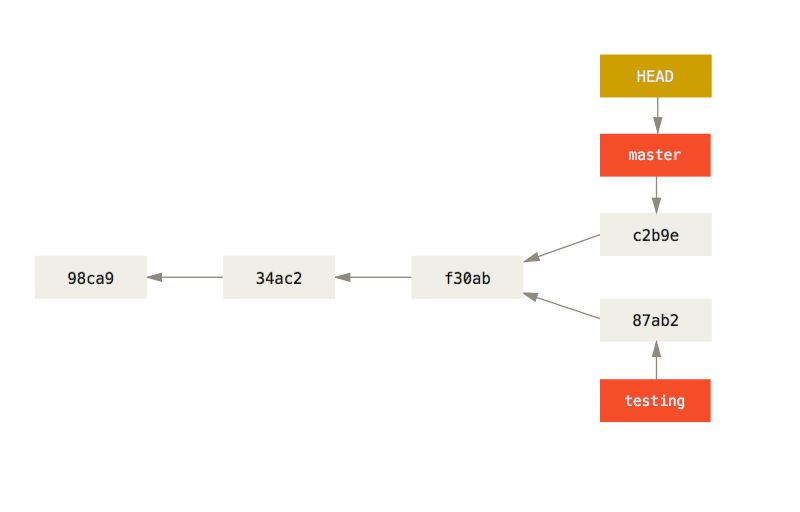
\includegraphics[width=\linewidth]{figures/advance-master}
  \end{center}
\end{frame}


\defverbatim[colored]\gitten{
  \begin{shcode}
      $ gedit ...
      $ git commit -m "My change to the special branch" -a
      $ git log --oneline #has the new commit
      ...
      $ git log --oneline master #as before
      ...
      $ git checkout master #To go back to the master
      $ git merge testing #To merge all changes back
      $ git branch -d testing #To remove the branch
  \end{shcode}
}
\begin{frame}
  \frametitle{Switching Branches: some commands}
  \vspace{2em}
  \gitten
\end{frame}

\defverbatim[colored]\giteleven{
  \begin{shcode}
      $ git branch old-release tag-1.2.4
      $ git checkout old-release #state of version 1.2.4
      # edit the changes
      $ git commit -m "..."
      # release version 1.2.5 from that point
  \end{shcode}
}

\begin{frame}
  \frametitle{How to Properly Use Tag/Branches}

  As rule of thumb:

  \vspace{1em}

  \begin{itemize}
    \item Everytime you make a \textbf{new release}, you \textbf{tag} your
      repository so you know what was distributed
    \item You use branches to:
      \begin{itemize}
        \item Test new features w/o disturbing the stability of \texttt{master}
        \item Fix problems with old versions of the software:

          \vspace{1em}
          \giteleven
      \end{itemize}
  \end{itemize}
\end{frame}
